\chapter{From Neutron stars to Kilonova}\label{chap:BNMS}

Kilonovae is going to be our main topic of study through the whole thesis.
Every chapter and section was build with the objective to develop the intuition on all the processes that takes part in the kilonova.
We will first present the neutron star with its dense matter in the general relativity description. 
The we will move to the problem of finding two neutron star in a close orbit and present a little discussion on why the existing of such configurations are not trivial.
Then we will describe the different phases of the merger with the different mechanism of emission, gravitational waves, short gamma ray bursts and our favorite the kilonova.
We will conclude with a detailed and current understanding of this last one. 
\section{The Neutron star}\label{NS}
Neutron stars contain the densest matter known to exist in a stable state. 
In their outer layers, nuclei coexist with a degenerate electron gas. 
With increasing density, electron captures make the nuclei progressively more neutron-rich until, at the neutron-drip density $n_{\rm drip}\simeq 2.5\times10^{-4}~\mathrm{fm^{-3}}$ ($\rho\simeq 4\times10^{11}~\mathrm{g\,cm^{-3}}$), neutrons are no longer bound to the nuclei and form a free neutron gas~\cite{baym_neutron_1971}.
At about half the saturation density the difference between inside and outside of a nucleus vanish effectively becoming a continuum of nucleons which marks the transition from crust to core.
Their core can reach several times the nuclear saturation density $n_{\rm sat}\simeq 0.15~\mathrm{fm^{-3}}$~\cite{horowitz_insights_2020}. 
At the same time the $\beta$ equilibrium favors neutrons instead of protons, this leads to a neutron dominated composition.  

Their hydrostatic equilibrium is determined by the equation of state (EOS) through the Tolman-Oppenheimer-Volkoff equations plus rotational corrections.
A free, degenerate neutron gas can support stars of at most $\simeq 0.7\,M_\odot$ \cite{oppenheimer_massive_1939}.
But, since the matter inside the star is expected to be dominated by neutrons really close to each other, the EOS will have to account the interactions between neutrons.
At such densities neutrons interact strongly and experiments a repulsive short-range interaction, which in relativistic mean-field models is mediated by $\omega$-meson exchange. 
Through this link between microphysics and astrophysical observables, neutron stars have become natural laboratories for strongly interacting matter at densities that cannot be reached in terrestrial experiments.

However the microscopic theory of this matter, quantum chromodynamics (QCD), cannot at present provide a complete description of the EOS in the relevant density range.
This is because at the baryon chemical potentials of neutron-star cores, QCD is non-perturbative, and lattice QCD is hampered by the fermion sign problem at finite baryon density. 
Controlled calculations exist only in two limits, chiral effective field theory describes nuclear matter up to about $1$-$2\,n_{\rm sat}$ \cite{hebeler_equation_2013}, and perturbative QCD becomes reliable only at densities of order $40\,n_{\rm sat}$, far above those realized in neutron stars \cite{kurkela_constraining_2014}.
In the intermediate regime, where neutron-star cores reside, the EOS is described by phenomenological models whose predictions must be confronted with astrophysical observations.

As a consequence, a description from first principles of neutron star cores remains unknown.
Matter at several times $n_{\rm sat}$ may consist of nucleons, may contain hyperons, or may undergo a transition to deconfined quark matter, either through a smooth crossover or through a first order hadron-quark phase transition \cite{baym_hadrons_2018}.

\section{Formation of binary neutron stars that merge}\label{sec:formation}

For two neutron stars to merge, three conditions must be met.
Both stars must form, which requires two core-collapse supernovae so the binary must survive both explosions.
Then the two remnants must end up close enough for gravitational-wave (GW) emission to bring them into contact in less than a Hubble time.
For typical neutron-star masses, the initial separation must be smaller than about $5\,R_\odot$.
This is two to three orders of magnitude smaller than the radii that the progenitor stars reach as supergiants.
The central problem of binary-neutron-star formation is therefore how to bring the compact remnants of two massive stars to separations far smaller than the stars themselves once were, without unbinding the system on the way.

In the standard isolated channel, a double neutron star (DNS) descends from a binary of two OB stars that are massive enough to end their lives in a core-collapse SN, see figure \ref{fig:DNS formation}.
If the initial binary are separated enough the descending DNS will not be close enough to merge.
If, on the contrary, the initial star are close, they will interact via stable or unstable mass transfer. 
Once one of the stars reach the end of its live the star will expands transferring part of its mass to their companion. 
If after the supernova the two stars remain bounded they will become a high-mass X-ray binary (HMXB).
When the second star expands it will bolt the first star in a phase called common envelope \cite{paczynski_common_1976}. 
In that stage the dynamical friction of the motion of the first star inside the second one will cause the necessary loss of angular momentum to bring closer the cores.
This phase is not stable so eventually the envelope will fall to the stars ofr get ejected leaving behind the first NS and the He core of the second one that eventually will die in what is called a ultra-strippend SN \cite{tauris_erratum_2017}.
finally the system will results in a DNS close enough to merge.
The sequence of events is reviewed in \cite{tauris_formation_2017}.
 
%%%%%%%%%%%%%%%%%  begin figure  %%%%%%%%%%%%%%%%%%%%%%%%%%%
\begin{figure}[t]
    \centering
    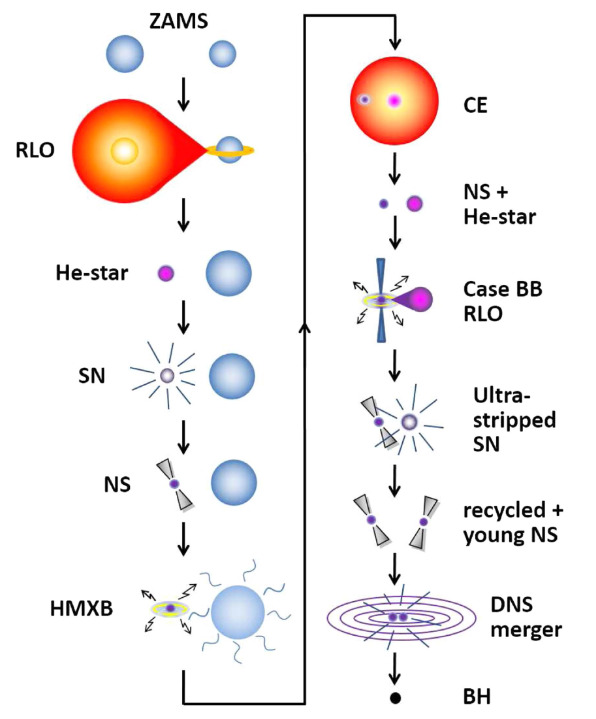
\includegraphics[width=0.7\textwidth]{Figures/DNS_formation.jpeg}    
    \caption{Double neutron star (DNS) formation from two OB stars as presented in \cite{tauris_formation_2017}. ZAMS refers to zero-age main sequence, RLO roche lobe overflow, SN supernova, HMXB high mass X ray binary and CE common envelope}
    \label{fig:DNS formation}
\end{figure}
%%%%%%%%%%%%%%%%%%%  end figure  %%%%%%%%%%%%%%%%%%%%%%%%%%%%%

\section{Gravitational-wave-driven inspiral and the maximum separation}\label{sec:formation-gw}
 
Once both neutron stars have formed, the only process that changes the orbit appreciably is the emission of gravitational radiation.
Here I will show an estimate of the time to the merger at leading (quadrupole) order and the maximum initial separation that allows a merger within the age of the Universe.

Consider two point masses $m_1$ and $m_2$ on a circular orbit of separation $a$ and angular frequency $\omega$, with total mass $M = m_1 + m_2$ and reduced mass $\mu = m_1 m_2 / M$.
Kepler's third law gives $\omega^{2} = GM/a^{3}$. 
In the centre of mass frame, the relative coordinate is $\mathbf{x}(t) = a\,(\cos\omega t, \sin\omega t, 0)$, and the trace-free mass quadrupole is $Q_{ij} = \mu\,(x_i x_j - \tfrac{1}{3}\delta_{ij} a^{2})$.
Its time-dependent components oscillate at $2\omega$:
\begin{equation}
  Q_{xx} = -Q_{yy} = \frac{\mu a^{2}}{2}\cos 2\omega t + \text{const}, \qquad
  Q_{xy} = \frac{\mu a^{2}}{2}\sin 2\omega t .
\end{equation}
The quadrupole formula~\cite{peters_gravitational_1964},
\begin{equation}
  L_{\rm GW} = \frac{G}{5c^{5}}\left\langle \dddot{Q}_{ij}\dddot{Q}_{ij}\right\rangle,
\end{equation}
with $\dddot{Q}_{xx}^{2} + \dddot{Q}_{yy}^{2} + 2\dddot{Q}_{xy}^{2}
= 32\,\mu^{2} a^{4}\omega^{6}$, gives the GW luminosity
\begin{equation}\label{eq:lgw}
  L_{\rm GW} = \frac{32}{5}\frac{G}{c^{5}}\mu^{2}a^{4}\omega^{6}
             = \frac{32}{5}\frac{G^{4}}{c^{5}}\frac{(m_1 m_2)^{2} M}{a^{5}} .
\end{equation}
The energy radiated is drawn from the orbital energy
$E = -G m_1 m_2/(2a)$. Setting $\mathrm{d}E/\mathrm{d}t = -L_{\rm GW}$
gives
\begin{equation}\label{eq:dadt}
  \frac{\mathrm{d}a}{\mathrm{d}t} = -\frac{\beta}{a^{3}}, \qquad
  \beta \equiv \frac{64}{5}\frac{G^{3} m_1 m_2 M}{c^{5}} .
\end{equation}
Equation~\eqref{eq:dadt} integrates to $a^{4}(t) = a_0^{4} - 4\beta t$,
so a binary with initial separation $a_0$ coalesces ($a \to 0$) after
\begin{equation}\label{eq:tc}
  t_{\rm c}(a_0) = \frac{a_0^{4}}{4\beta}
  = \frac{5}{256}\frac{c^{5} a_0^{4}}{G^{3} m_1 m_2 M} .
\end{equation}
The steep $a_0^{4}$ dependence is the key point. Halving the separation
shortens the inspiral by a factor of sixteen.

Now lets estimate the maximum separation for BNS to merger within the age of the universe.
Notice that since the stars require a preliminary formation and evolution we will therefore over estimate the maximum distances between stars.
Lets require $t_{\rm c} \le t_{\rm H}$, with $t_{\rm H} \simeq 13.8~\mathrm{Gyr}$ the age of the Universe
\begin{equation}\label{eq:amax}
  a_{\max} = \left(4\beta\, t_{\rm H}\right)^{1/4}
  = \left(\frac{256}{5}\frac{G^{3} m_1 m_2 M}{c^{5}}\, t_{\rm H}\right)^{1/4} .
\end{equation}
For $m_1 = m_2 = 1.35\,M_\odot$, the configuration simulated in this work,
$m_1 m_2 M = 4.92\,M_\odot^{3}$ and
$\beta = 6.08\times10^{27}~\mathrm{cm^{4}\,s^{-1}}$. Hence
\begin{equation}\label{eq:amax-num}
  a_{\max} \simeq 3.2\times10^{6}~\mathrm{km}
  \left(\frac{t}{13.8~\mathrm{Gyr}}\right)^{1/4}
  \left(\frac{m_1 m_2 M}{4.92\,M_\odot^{3}}\right)^{1/4}
  \simeq 4.6\,R_\odot ,
\end{equation}
about $0.02~\mathrm{AU}$. By Kepler's third law, this corresponds to a
maximum orbital period $P_{\max} \simeq 17~\mathrm{h}$. Equivalently, in
terms of the orbital period and the chirp mass
$\mathcal{M} = (m_1 m_2)^{3/5}/M^{1/5}$,
\begin{equation}\label{eq:tc-period}
  t_{\rm c} = \frac{5}{256}\left(\frac{G\mathcal{M}}{c^{3}}\right)^{-5/3}
  \left(\frac{P}{2\pi}\right)^{8/3}
  \simeq 13.8~\mathrm{Gyr}
  \left(\frac{P}{16.8~\mathrm{h}}\right)^{8/3}
  \left(\frac{\mathcal{M}}{1.175\,M_\odot}\right)^{-5/3} .
\end{equation}
Two consistency checks are worth noting. At $a_{\max}$, the orbital
velocity is $v/c = (GM/a_{\max}c^{2})^{1/2} \approx 10^{-3}$, so
post-Newtonian corrections of relative order $(v/c)^{2} \sim 10^{-6}$ are
negligible over almost the entire inspiral. They become important only in
the last orbits. At the initial separation of the simulation in this work
(45~km), the post-Newtonian expansion parameter is
$x = (GM\omega/c^{3})^{2/3} \approx 0.09$, and the final orbits and the
merger require a full numerical solution of the Einstein equations
(Chapter~\ref{ch:numerical}). Tidal effects are likewise negligible until
the separation is a few stellar radii.
